\section{割线条件}
\label{sec:qn-secant}

不计算Hessian，单凭已经读到的梯度，能知道多少曲率？答案是一条线性方程组，它精确地说出了一次测量包含的信息，也说明了这些信息还远远不够。

\paragraph{用近似矩阵代替Hessian}
Newton法在当前点$\bm{x}^{(t)}$处用二次模型近似目标。把模型里的Hessian换成一个对称矩阵$\bm{B}^{(t)}$，模型变成
\begin{equation}
 m^{(t)}(\bm{p})=f(\bm{x}^{(t)})+\langle\bm{g}^{(t)},\bm{p}\rangle+\frac12\bm{p}^\top\bm{B}^{(t)}\bm{p}.
 \label{eq:qn-model}
\end{equation}
当$\bm{B}^{(t)}$正定时，模型是严格凸的，令它的梯度$\bm{g}^{(t)}+\bm{B}^{(t)}\bm{p}$为零，得到唯一极小点
\begin{equation}
 \bm{d}^{(t)}=-\bm{W}^{(t)}\bm{g}^{(t)},\qquad\bm{W}^{(t)}=\bigl(\bm{B}^{(t)}\bigr)^{-1}.
 \label{eq:qn-direction}
\end{equation}
这里$\bm{B}^{(t)}$叫曲率近似，$\bm{W}^{(t)}$叫逆曲率近似。全卷$\bm{H}^{(t)}$专指真实Hessian，所以逆近似用$\bm{W}$表示。下面只需要回答一件事：这两个矩阵从哪里来。

\paragraph{一维情形：割线}
先看只有一个变量的目标。设$f(x)=\tfrac14x^4+\tfrac12x^2$，梯度$g(x)=x^3+x$，已经走过$x^{(0)}=1$和$x^{(1)}=0.5$，读到
\[
 g(x^{(0)})=2,\qquad g(x^{(1)})=0.625.
\]
过这两点作$g$的割线，斜率是
\[
 b=\frac{g(x^{(1)})-g(x^{(0)})}{x^{(1)}-x^{(0)}}=\frac{0.625-2}{0.5-1}=2.75.
\]

这个斜率介于两端的真实二阶导数$f''(0.5)=1.75$与$f''(1)=4$之间。由微积分基本定理，它正好是$f''$在这一段上的平均值。把$b$当作曲率，下一个点就是割线与横轴的交点：
\[
 x^{(2)}=x^{(1)}-\frac{g(x^{(1)})}{b}=0.5-\frac{0.625}{2.75}\approx0.273.
\]
图~\ref{fig:qn-secant-1d}画出了这一步。割线不如切线精确，却不需要二阶导数，只用两次已经算过的梯度。

\begin{BookInlineFigure}
  \centering
  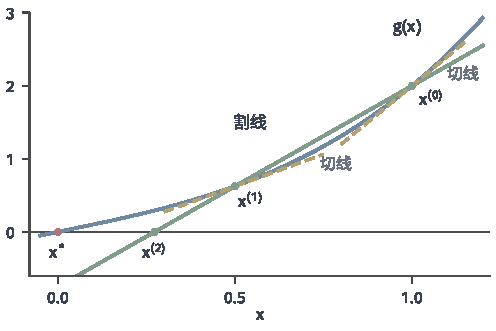
\includegraphics[width=84mm]{figures/05-optimization/02-smooth-optimization/matplotlib/qn-secant-1d/figure.pdf}
  \caption{一维的割线步。蓝线是$f(x)=\tfrac14x^4+\tfrac12x^2$的梯度$g(x)=x^3+x$。绿线是过$x^{(0)}=1$、$x^{(1)}=0.5$两点的割线，斜率$2.75$是$f''$在这一段的平均值；两条黄色虚线是两端的切线，斜率分别为$4$和$1.75$。割线与横轴的交点给出下一个迭代点$x^{(2)}\approx0.273$，红点是最优解。}
  \label{fig:qn-secant-1d}
\end{BookInlineFigure}

\paragraph{高维情形：梯度差是平均曲率作用于位移}
高维时除法做不了，但关系仍在。记位移与梯度差分别为
\begin{equation}
 \bm{s}^{(t)}=\bm{x}^{(t+1)}-\bm{x}^{(t)},\qquad\bm{y}^{(t)}=\bm{g}^{(t+1)}-\bm{g}^{(t)}.
 \label{eq:qn-s-y}
\end{equation}
沿线段$\bm{x}^{(t)}+\tau\bm{s}^{(t)}$（$\tau\in[0,1]$）对梯度用微积分基本定理，得到
\begin{equation}
 \bm{y}^{(t)}=\bar{\bm{H}}^{(t)}\bm{s}^{(t)},\qquad
 \bar{\bm{H}}^{(t)}=\int_0^1\nabla^2f\bigl(\bm{x}^{(t)}+\tau\bm{s}^{(t)}\bigr)\,\mathrm{d}\tau.
 \label{eq:qn-average-hessian}
\end{equation}
所以$\bm{y}^{(t)}$是这一段路上的平均Hessian作用在位移上的结果。对二次目标，Hessian是常数$\bm{A}$，等式成为精确的$\bm{y}^{(t)}=\bm{A}\bm{s}^{(t)}$。

可以把每一步想成一次路试。车沿某条路开过去，记下坡度的变化，就知道这条路上地形弯得多厉害。对应关系是：路线对应$\bm{s}^{(t)}$，坡度变化对应$\bm{y}^{(t)}$，弯曲程度对应$\bar{\bm{H}}^{(t)}$在这个方向上的作用。

这个类比有两处要小心。一次路试只告诉我们沿路线方向的信息，与路线垂直的方向几乎没有测量；地形不是二次的时候，旧路试测到的曲率会随着位置改变而过时。

既然模型要代表目标在下一个点的局部形状，自然要求新的矩阵重现最新的测量。

\begin{definition}[割线条件]
\label{def:qn-secant}
给定$\bm{s}^{(t)}$与$\bm{y}^{(t)}$，称对称矩阵$\bm{B}^{(t+1)}$满足\term{割线条件}（secant condition），如果
\begin{equation}
 \bm{B}^{(t+1)}\bm{s}^{(t)}=\bm{y}^{(t)}.
 \label{eq:qn-secant}
\end{equation}
用逆曲率近似$\bm{W}^{(t+1)}$表示时，条件写成
\begin{equation}
 \bm{W}^{(t+1)}\bm{y}^{(t)}=\bm{s}^{(t)}.
 \label{eq:qn-secant-inverse}
\end{equation}
\end{definition}

割线条件有一个几何含义。以$\bm{x}^{(t+1)}$为中心的模型在新点的梯度是$\bm{g}^{(t+1)}$，在旧点（$\bm{p}=-\bm{s}^{(t)}$）的梯度是
\[
 \bm{g}^{(t+1)}-\bm{B}^{(t+1)}\bm{s}^{(t)}=\bm{g}^{(t+1)}-\bm{y}^{(t)}=\bm{g}^{(t)}.
\]
也就是说，模型在新旧两点的梯度都与目标一致。使用满足割线条件的矩阵，并按这种方式选择方向的方法统称\term{拟牛顿法}（quasi-Newton method）。

下面用贯穿例算出第一组测量。取$\bm{W}^{(0)}=\bm{I}$，第一步就是负梯度方向。在二次目标上，沿方向$\bm{d}$的精确线搜索步长是
\[
 \alpha=\frac{-\langle\bm{g},\bm{d}\rangle}{\bm{d}^\top\bm{A}\bm{d}}.
\]
代入第一轮的数据，得到
\[
 \bm{g}^{(0)}=(8,8)^\top,\qquad\bm{d}^{(0)}=(-8,-8)^\top,\qquad\alpha^{(0)}=\frac{128}{640}=\frac15.
\]

走完这一步，得到新的点和梯度：
\[
 \bm{x}^{(1)}=(2.4,-0.6)^\top,\qquad\bm{g}^{(1)}=(4.8,-4.8)^\top.
\]
位移和梯度差是
\begin{equation}
 \bm{s}^{(0)}=(-1.6,-1.6)^\top,\qquad\bm{y}^{(0)}=(-3.2,-12.8)^\top.
 \label{eq:qn-running-pair}
\end{equation}

\paragraph{一条割线条件定不出矩阵}
割线条件有$n$个方程，对称矩阵有$n(n+1)/2$个自由元素，还差$n(n-1)/2$个条件。$n=1$时恰好相等，这正是一维割线法没有选择余地的原因。$n$一大，缺口迅速变大。

图~\ref{fig:qn-secant-unknowns}说明缺的是哪些信息。把$\bm{s}$单位化后作为第一个基向量。$\bm{B}\bm{s}=\bm{y}$确定了矩阵的第一列，对称性再确定第一行，其余$(n-1)\times(n-1)$的对称块完全自由。换句话说，矩阵在与$\bm{s}$正交的子空间内怎样弯曲，这次路试没有提供任何信息。

\begin{BookInlineFigure}
  \centering
  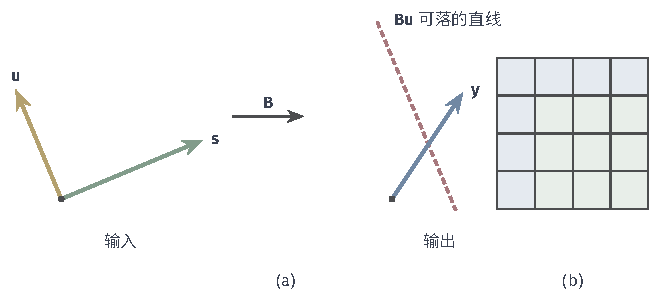
\includegraphics[width=110mm]{figures/05-optimization/02-smooth-optimization/tikz/qn-secant-unknowns/figure.pdf}
  \caption{割线条件确定了矩阵的哪些部分。(a)$n=2$时，$\bm{B}$把$\bm{s}$送到已知的$\bm{y}$；对另一个方向$\bm{u}$，对称性只给出$\langle\bm{Bu},\bm{s}\rangle=\langle\bm{u},\bm{y}\rangle$，所以$\bm{Bu}$只知道落在红色虚线上。(b)$n=4$时，在以$\bm{s}$为第一个基向量的正交基下，蓝色的第一行第一列由割线条件和对称性确定，绿色的$3\times3$对称块的$6$个元素仍然自由。}
  \label{fig:qn-secant-unknowns}
\end{BookInlineFigure}

用贯穿例看得更具体。设$\bm{B}=\begin{bmatrix}a&b\\b&c\end{bmatrix}$，把式~\eqref{eq:qn-running-pair}代入割线条件，两个方程约去公因子后是
\[
 a+b=2,\qquad b+c=8.
\]
三个未知数、两个方程，还剩一个自由参数：
\begin{equation}
 \bm{B}(a)=\begin{bmatrix}a&2-a\\2-a&6+a\end{bmatrix},\qquad
 \det\bm{B}(a)=10a-4.
 \label{eq:qn-secant-family}
\end{equation}
真实Hessian是其中$a=2$的成员，但算法无从知道。

族中不同成员给出的方向也不同。若第一步取较短的步长$\alpha^{(0)}=1/8$，位移与梯度差只差一个倍数，方程不变，于是仍是族~\eqref{eq:qn-secant-family}。此时$\bm{x}^{(1)}=(3,0)^\top$，$\bm{g}^{(1)}=(6,0)^\top$，方向$-\bm{B}(a)^{-1}\bm{g}^{(1)}$的计算结果是
\[
 \begin{aligned}
 a=0.9:&\quad(-8.28,\ 1.32)^\top,\\
 a=2:&\quad(-3,\ 0)^\top,\\
 a=5:&\quad(-1.435,\ -0.391)^\top.
 \end{aligned}
\]

只有$a=2$的方向一步落到最优解。图~\ref{fig:qn-secant-family}(a)把这些模型画在一起：它们在$\bm{x}^{(0)}$处都与同一条红色切线相切，这是割线条件保证的，在别的地方却差别很大，极小点也各不相同。

\begin{BookInlineFigure}
  \centering
  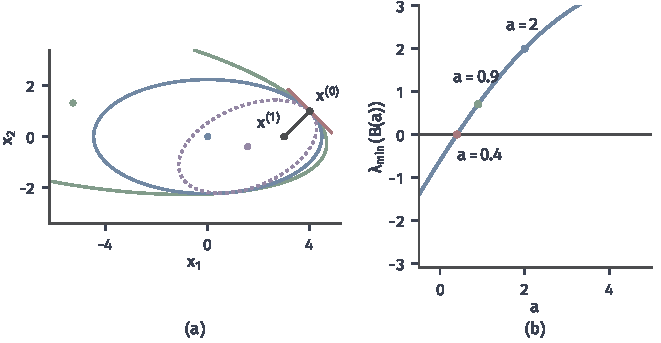
\includegraphics[width=112mm]{figures/05-optimization/02-smooth-optimization/matplotlib/qn-secant-family/figure.pdf}
  \caption{满足同一割线条件的矩阵族~\eqref{eq:qn-secant-family}。(a)从$\bm{x}^{(0)}=(4,1)$走到$\bm{x}^{(1)}=(3,0)$后，$a=0.9$（绿）、$a=2$（蓝）、$a=5$（紫，点线）三个模型过$\bm{x}^{(0)}$的等值线，它们在$\bm{x}^{(0)}$处有同一条切线（红），同色小点是各模型的极小点。(b)$\bm{B}(a)$的最小特征值，$a>0.4$时为正。}
  \label{fig:qn-secant-family}
\end{BookInlineFigure}

\paragraph{还要补充什么要求}
既然割线条件不够，就要额外规定想要什么样的矩阵。后面各种方法的区别，就在这些补充要求上。

第一是\textbf{对称}。Hessian对称，近似矩阵也应该对称，这已经写进了定义。

第二是\textbf{低秩修正}：$\bm{B}^{(t+1)}$与$\bm{B}^{(t)}$只差一个秩很低的矩阵。这样做既保留了以前路试积累的信息，也使更新只花$O(n^2)$次运算。它还能配合逆矩阵的公式，直接更新$\bm{W}$，于是根本不用解线性方程。

第三是\textbf{曲率性质}。我们希望$\bm{B}^{(t+1)}$正定，这样方向~\eqref{eq:qn-direction}才是模型的极小点。但正定性对测量数据有要求。用$\bm{s}^{(t)}$与割线条件~\eqref{eq:qn-secant}作内积，得到
\begin{equation}
 \bigl(\bm{s}^{(t)}\bigr)^\top\bm{B}^{(t+1)}\bm{s}^{(t)}=\langle\bm{s}^{(t)},\bm{y}^{(t)}\rangle.
 \label{eq:qn-curvature-identity}
\end{equation}
左边在$\bm{B}^{(t+1)}\succ\bm{0}$且$\bm{s}^{(t)}\neq\bm{0}$时为正，所以必须有
\begin{equation}
 \langle\bm{s}^{(t)},\bm{y}^{(t)}\rangle>0.
 \label{eq:qn-curvature-condition}
\end{equation}
这个不等式称为\term{曲率条件}（curvature condition）。它的含义是：沿刚走过的路，平均来看地形向上弯。

曲率条件确实可能不成立。取不定的二次目标，其Hessian为$\operatorname{diag}(2,-1)$，$\bm{s}=(1,2)^\top$，则
\[
 \bm{y}=(2,-2)^\top,\qquad\langle\bm{s},\bm{y}\rangle=2-4=-2<0.
\]
这时任何满足割线条件的矩阵都不可能正定。曲率条件是必要条件，第~\ref{sec:qn-dfp-bfgs}节将说明，配合恰当的更新，它也是充分的。

\paragraph{接入线搜索}
得到$\bm{W}^{(t)}$后，拟牛顿法沿用第~\ref{chap:smooth-foundations}章的线搜索框架：
\begin{equation}
 \bm{x}^{(t+1)}=\bm{x}^{(t)}+\alpha^{(t)}\bm{d}^{(t)},\qquad\bm{d}^{(t)}=-\bm{W}^{(t)}\bm{g}^{(t)}.
 \label{eq:qn-iteration}
\end{equation}
只要$\bm{W}^{(t)}$正定且$\bm{g}^{(t)}\neq\bm{0}$，就有
\[
 \langle\bm{g}^{(t)},\bm{d}^{(t)}\rangle=-\bigl(\bm{g}^{(t)}\bigr)^\top\bm{W}^{(t)}\bm{g}^{(t)}<0,
\]
方向是下降方向，线搜索一定能找到使目标下降的步长。

步长的试探从$\alpha=1$开始，因为$\bm{d}^{(t)}$本身是模型的极小点，近似矩阵好的时候它就是合适的长度。常用的接受标准是Wolfe条件：取$0<c_1<c_2<1$，要求$\alpha$同时满足充分下降和曲率两条不等式，
\begin{equation}
 \begin{aligned}
 f(\bm{x}^{(t)}+\alpha\bm{d}^{(t)})&\leq f(\bm{x}^{(t)})+c_1\alpha\langle\bm{g}^{(t)},\bm{d}^{(t)}\rangle,\\
 \langle\nabla f(\bm{x}^{(t)}+\alpha\bm{d}^{(t)}),\bm{d}^{(t)}\rangle&\geq c_2\langle\bm{g}^{(t)},\bm{d}^{(t)}\rangle.
 \end{aligned}
 \label{eq:qn-wolfe}
\end{equation}
第一条不让步长过长，第二条不让步长过短。第~\ref{chap:smooth-foundations}章已经说明，下降方向上目标有下界时，这样的步长总是存在。第二条在这里还有一个专门的用途，下一节会看到。

把三类方向放在一起，能看清拟牛顿法的位置。它们的区别不在迭代的形式，而在第一项的矩阵由什么信息构成。

\begin{BookInlineTable}
  \centering
  \begin{tabular}{llll}
    \toprule
    方法 & 方向 & 用到的信息 & 每步新增的曲率信息\\
    \midrule
    梯度下降 & $-\bm{g}^{(t)}$ & 梯度 & 无\\
    拟牛顿法 & $-\bm{W}^{(t)}\bm{g}^{(t)}$ & 梯度与历史 & 一次沿位移的测量\\
    Newton法 & $-(\bm{H}^{(t)})^{-1}\bm{g}^{(t)}$ & 梯度与Hessian & 完整的曲率\\
    \bottomrule
  \end{tabular}
  \caption{三类方向的对比。}
  \label{tab:qn-direction-comparison}
\end{BookInlineTable}
